%!TEX root = ./Thesis.tex

\chapter{Introduction}
\label{chapter:introduction}

\section{Quantum information science}

\tmpHeading{What is quantum information?}
% Quantum information science studies how information behaves, and can be manipulated, at the quantum level~\cite{nielsen2006quantum,watrous2018theory} \highlight{(rifare}).
Quantum mechanics has profound implications for our understanding of how information can be manipulated.
This has clear and far-reaching consequences both from a fundamental perspective, and for its potential to improve existing information technologies.
\emph{Quantum information science} studies this merger of the fields of quantum mechanics and information and computational theory~\cite{nielsen2006quantum,watrous2018theory}.
% \emph{Quantum information science} studies the ways quantum mechanics can improve information processing tasks.
% Quantum information science studies the implications of quantum mechanics to our understanding of how information can be manipulated.
The subject focuses not only on devising protocols to achieve faster information processing, but also promises faster and more secure communication protocols~\cite{gisin2002quantum,krenn2016quantum,pirandola2019advances}.
Among the many approaches explored in the course of the last fifty years, arguably the most notable areas of research fall under the names of quantum computation~\cite{shor1997polynomial,steane1998quantum,ladd2010quantum,wolf2019quantum}, quantum simulation~\cite{lloyd1996universal,georgescu2014quantum,koch2019quantum}, quantum communication~\cite{bennett1993teleporting,gisin2007quantum,krenn2016quantum}, and quantum cryptography~\cite{gisin2002quantum,bennett2014quantum}.


\tmpHeading{Quantum computing}
Quantum computation, in particular, holds the promise of solving efficiently classically hard computational problems.
Ever since Feynman first proposed to use quantum mechanics to simulate efficiently quantum systems~\cite{feynman1982simulating}, more and more research has been devoted to understanding why and how quantum mechanics provides computational advantages.
% The realisation that this was possible at all prompted a shift of interest into a broad variety of research directions, focused on applying quantum mechanics to improve various technologies. This is sometimes referred to as a \textit{second quantum revolution}~\cite{dowling2003quantum}.
Still, the dream of practical and useful quantum computation remains far on the horizon, and arguably still requires a number of theoretical and technological advances~\cite{dowling2003quantum,preskill2018quantum},
despite recent years having seen an substantial number of breakthroughs~\cite{fowler2012surface,barends2014superconducting,córcoles2015demonstration,ofek2016extending,arute2019quantum}.
Even though scalable and fault-tolerant quantum computation remains a titanic challenge with present-day technology, there are ways to at least settle the overarching question of whether it is possible \textit{even in principle} to solve problems faster than what classical physics allows~\cite{aaronson2011computational,bremner2016average,boixo2018characterizing,aaronson2017complexity,neill2018blueprint}. This spurred the race to reach the so-called \textit{quantum computational supremacy} regime, that is, to demonstrate experimentally the solution to a problem that is computationally hard for classical computers, regardless of its practical usefulness~\cite{broome2012photonic,spring2012boson,crespi2013integrated,tillmann2013experimental,bentivegna2015experimental,zhong201812photon,zhong2019experimental,wang2019boson,bouland2018complexity,arute2019quantum}.
Several architectures have been proposed as possible physical carriers of quantum information, including schemes relying on photonics~\cite{flamini2018photonic,wang2019integrated}, trapped ions and cold atoms~\cite{garcía-ripoll2005quantum,lekitsch2017blueprint,bruzewicz2019trappedion}, and superconducting technologies~\cite{you2011atomic,krantz2019quantum}
Similarly, different paradigms for quantum computation have been developed. One broad distinction can be made between \textit{discrete variables}~\cite{walmsley2005applied,andersen2015hybrid} and \textit{continuous variables}~\cite{lloyd1999quantum,braunstein2005quantum} approaches.
Another important distinction is between different computational models, ranging from the circuit model~\cite{nielsen2006quantum}, to one-way quantum computation~\cite{raussendorf2001one,walther2005experimental,browne2006one}, to adiabatic quantum computing~\cite{aharonov2004adiabatic,albash2018adiabatic}.

\tmpHeading{How are we connected to the problems in quantum computing?}
In this thesis, we will discuss questions arising in different areas of quantum information processing.
In particular, we consider in~\cref{chapter:gate_learning} the task of devising dynamics resulting in target operations between a set of qubits: the so-called \emph{quantum gate learning problem}.
We then discuss how to generate target quantum states leveraging a specific type of physical models, so-called \emph{quantum walks}, in~\cref{chapter:quantum_walks,chapter:experimental_engineering_qudits}.
Finally, in~\cref{chapter:ML_VVBs} we present a protocol to characterise generated quantum states from experimental data.

\section{Machine learning and quantum physics}
\label{sec:intro:ML}

\tmpHeading{Machine learning}
Parallel to the surge of interest in quantum technologies, another field of study that grew considerably in the last few decades is~\ac{ML}~\cite{friedman2001elements,you2011atomic,bishop2006pattern,abu2012learning,murphy2012machine,mehta2019highbias}.
\ac{ML} refers to a class of algorithms whose goal is to learn from, and make predictions about, data.
The underlying mathematical problem most of these algorithms tackle is to find a set of parameters $\bstheta$ such that the corresponding map $f_\bstheta:\bs x\mapsto f_\bstheta(\bs x)$ fits a given dataset, for some choice of \emph{model} $\bstheta\mapsto f_\bstheta$.
For example, in a \emph{classification problem}, $\bs x$ is a set of real numbers, and $f_\bstheta(\bs x)$ is chosen from a finite set of possible values.
% (for example, if we want to classify a set of images as representing ``cats'' or ``dogs'', $f_\bstheta(\bs x)\in\{\text{cat},\text{dog}\}$).

% \tmpHeading{ML and numerical optimisation}
% From this point of view, \ac{ML} algorithms might appear to be no different than simple fitting algorithms.
% % , and it is indeed not rare to hear people say that ``\emph{machine learning is just glorified curve-fitting}''.
% While this is somewhat true, in that both ``curve fitting'' and ``machine learning tasks'' can be unified under a single conceptual framework, such statements are off the mark when their implied meaning is to undersell the field of \ac{ML}.
% Indeed, the ``simple'' problem of ``fitting a model'' to a given dataset, when no further assumptions are made over the type of data and model, is such a generic and hard problem that vastly different techniques and ideas are required to handle it in different circumstances.

\tmpHeading{``Quantum machine learning''?}
The intersection of \ac{ML} and quantum information falls under the name of \ac{QML}~\cite{wittek2014quantum,schuld2014introduction,adcock2015advances,biamonte2017quantum}.
Due to the wide reach of both fields, \ac{QML} branches out into several different directions of study.
The terminology was first used to refer to quantum algorithms tackling \ac{ML} tasks~\cite{giovannetti2008quantum,harrow2009quantum,lloyd2013quantum,lloyd2014quantum,rebentrost2014quantum,lloyd2016quantum,rebentrost2018quantum,rebentrost2016quantum}.
% This line of study can also be considered as belonging to the fields of quantum computation and quantum algorithm development.
This line of study is now sometimes referred to as \emph{quantum-enhanced machine learning}~\cite{wittek2014quantum,schuld2014introduction,dunjko2017machine,ciliberto2018quantum,schuld2018supervised,perdomo-ortiz2018opportunities}.
Another direction of study, more focused on the theoretical foundations of \emph{learning} in a quantum mechanical context, is \emph{quantum learning theory}~\cite{aaronson2007learnability,aaronson2017shadow,arunachalam2017survey,aaronson2018online,rocchetto2019experimental}.
% \cite{giovannetti2008quantum,harrow2009quantum,sentís2012quantum,lloyd2013quantum,lloyd2014quantum,rebentrost2014quantum,wiebe2014quantum,aaronson2015read,sentís2015quantum,lloyd2016quantum,rebentrost2018quantum,schuld2016prediction,rebentrost2016quantum,childs2017quantum}.
Classical ML algorithms have also been used extensively to find solutions to problems arising in the context of quantum information science~\cite{zdeborov2017machine,spears2018deep,carleo2019machine}.
This latter topic is what a large part of this thesis will be devoted to.
% ############################# TO ADD BACK IF TIME ALLOWS
% \tmpHeading{Hybrid approaches}
% Hybrid classical-quantum approaches are also worth noting. Here we should cite works on VQA algorithms etc.

\tmpHeading{Machine learning for quantum information science}
Applications of classical ML to quantum information science include generating target quantum gates via supervised learning~\cite{banchi2016quantum}, finding physical models describing (simulated) experimental outcomes \cite{iten2020discovering,nautrup2020operationally}, probing characteristics of experimentally generated states~\cite{fujita2018construction,gray2018machinelearningassisted,havlíček2019supervised,canabarro2019machine,agresti2019pattern}, devising fault-tolerant and quantum error-correction schemes~\cite{liu2019neural},
using variational autoencoders to learn quantum distributions~\cite{rocchetto2018learning}, using reinforcement learning to devise sequences of operations resulting in target quantum protocols~\cite{melnikov2014projective,makmal2016metalearning,melnikov2017projective,melnikov2018benchmarking,melnikov2018active,wallnöfer2019machine,flamini2019photonic},
and using \acp{NN}-inspired ansatzes to find the ground state of many-body systems~\cite{carleo2017solving}, as well as a variety of other applications \cite{jia2019quantum,torlai2019integrating,cui2019directions,carleo2019machine}, including classifying phases in many-body systems~\cite{wang2016discovering,carrasquilla2017machine,van2017learning,deng2017machine,kaubruegger2018chiral}.
% \cite{torlai2017neural,torlai2017manybody,choo2018symmetries,saito2018method,torlai2018neuralnetwork,torlai2018latent,sharir2019deep,jia2019quantum,levine2019quantum,hartmann2019neuralnetwork,vicentini2019variational,torlai2019integrating,liu2019machine,harney2019entanglement,cui2019directions,carleo2019machine}.
% The expressive power of this \ansatz has also been explored~\cite{deng2017quantum,gao2017efficient}, as well as its connections with tensor networks~\cite{glasser2018neuralnetwork}.,


\tmpHeading{Supervised learning for quantum information science}
Supervised learning, in particular, provides powerful tools to extract patterns from labelled data.
In the context of quantum information, supervised learning has been showcased as a flexible tool to solve diverse complex optimisation tasks~\cite{zdeborov2017machine,carrasquilla2017machine,carleo2017solving,van2017learning,schoenholz2016structural,torlai2017manybody,rocchetto2019experimental,melnikov2018active,fujita2018construction}.
In particular, supervised learning techniques were recently demonstrated to solve \emph{gate design} problems~\cite{banchi2016quantum,innocenti2018supervised,innocenti2018approximate}.

\tmpHeading{How does all of this concern us?}
In this thesis, we will discuss ways to apply ML ideas to find solutions to problems arising in the context of theoretical and experimental quantum information.
In~\cref{chapter:gate_learning} we show how \emph{stochastic gradient descent} can be used to find time-independent dynamics generating target quantum gates.
In~\cref{chapter:ML_VVBs}, we use different ML algorithms to reconstruct the states underlying experimental datasets, making for more efficient and flexible experimental characterisation pipelines.


\section{Quantum walks}
\label{sec:intro:QWs}


% \tmpHeading{Classical RWs as stochastic processes}
% \acp{QW} have been introduced in 1993 by Aharonov et al.~\cite{aharonov1993quantum}.
% Konno proposed a solid mathematical connection between correlated \acp{QW} and another QW model~\cite{konno2003limit}.

\tmpHeading{Random walks}
Classical random walks are a class of stochastic processes used to develop stochastic algorithms, as well as in multiple other contexts~\cite{berg1993random,fama1995random,motwani1995randomized,hughes1996random,schoning1999probabilistic,codling2008random}.
A random walk is defined as a sequence of discrete \textit{steps} taken by a \textit{walker} in one of a number of allowed \emph{directions}~\cite{lovasz1993random}.
A common example are random walks on a \textit{regular lattice}. Here, the walking space is a regular $d$-dimensional lattice, which we can represent with $\ZZ^d$. The walker starts in a vertex $\bs n\in\ZZ^d$ and moves along the edges of the lattice.
At every step, one of the possible $2d$ directions (there are two directions for each axis) is picked at random, and the walker moves to the closest vertex along the corresponding edge.
One can define random walks more generally on undirected \textit{graphs}
\footnote{An \textit{directed simple graph} is a pair $G\equiv (V,E)$, where $V$ is a set of \textit{vertices}, and $E\subseteq V\times V$ is a subset of ordered pairs of $V$. When the edges $E$ do not carry a notion of directionality, being for example defined as $E=\{\{x,y\} : x,y\in V\text{ and }x\neq y\}$, then ones talks of an \textit{undirected} graph.}
, by having the walker jump at every step from one vertex to the other with some probability.
% Denoting with $v_t$ the position of the walker at the $t$-th step for some $t\in\NN$, the probability of finding the walker in the position $v_{t+1}$ at time $t+1$ is given by some probability $\Prob(v_{t+1}|v_{t})$. This is often referred to as the \emph{transition probability} of the random walk. 
% A crucial feature of the transition probabilities of quantum walks is that they are \emph{Markov chains}, that is, they only depend on the current state of the walker, as opposed to its whole history. \highlight{(is this last sentence necessary?)}
% The random walk is then defined by the set of \textit{transition probabilities} $p_{ij}$, which give the probability of a walker in the position $i$ at a time $t$ jumping into the position $j$ at time $t+1$.

% \begin{figure}[tb]
%     \centering
%     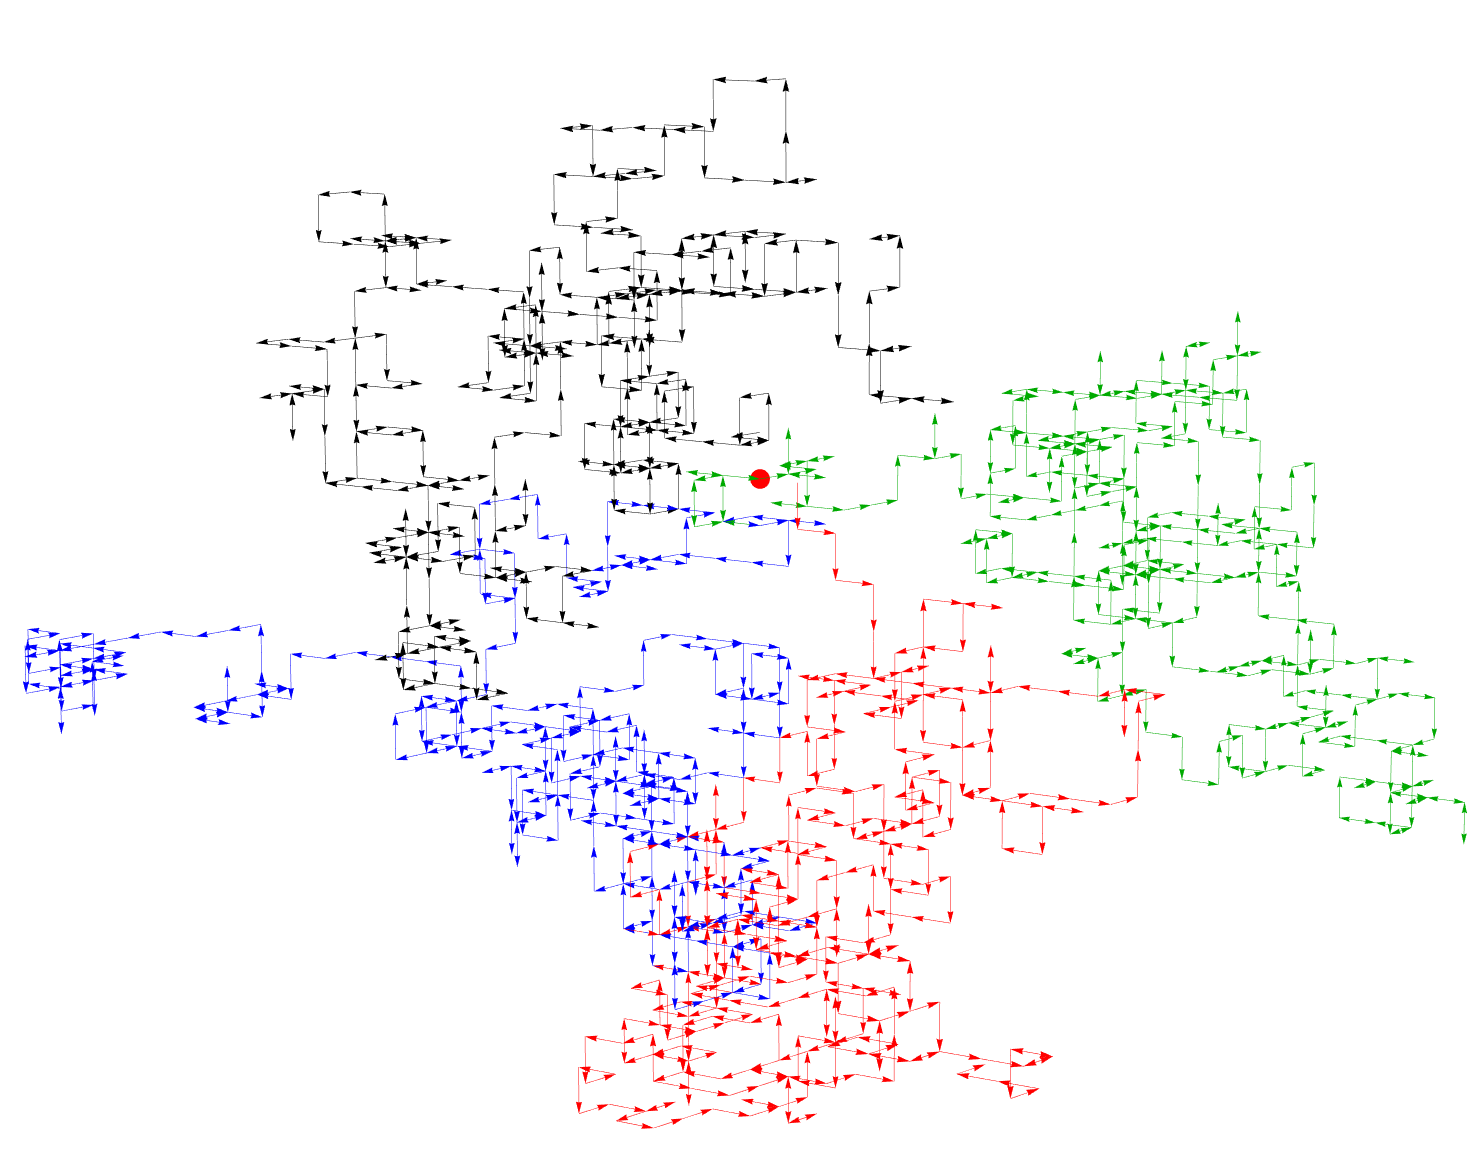
\includegraphics[width=0.8\linewidth]{Figures/quantum-walks/3d-randomwalk.png}
%     \caption{Example of three random walks on $\ZZ^3$.}
%     \label{fig:intro:3DQWs}
% \end{figure}
% \begin{wrapfigure}{r}{10cm}
%     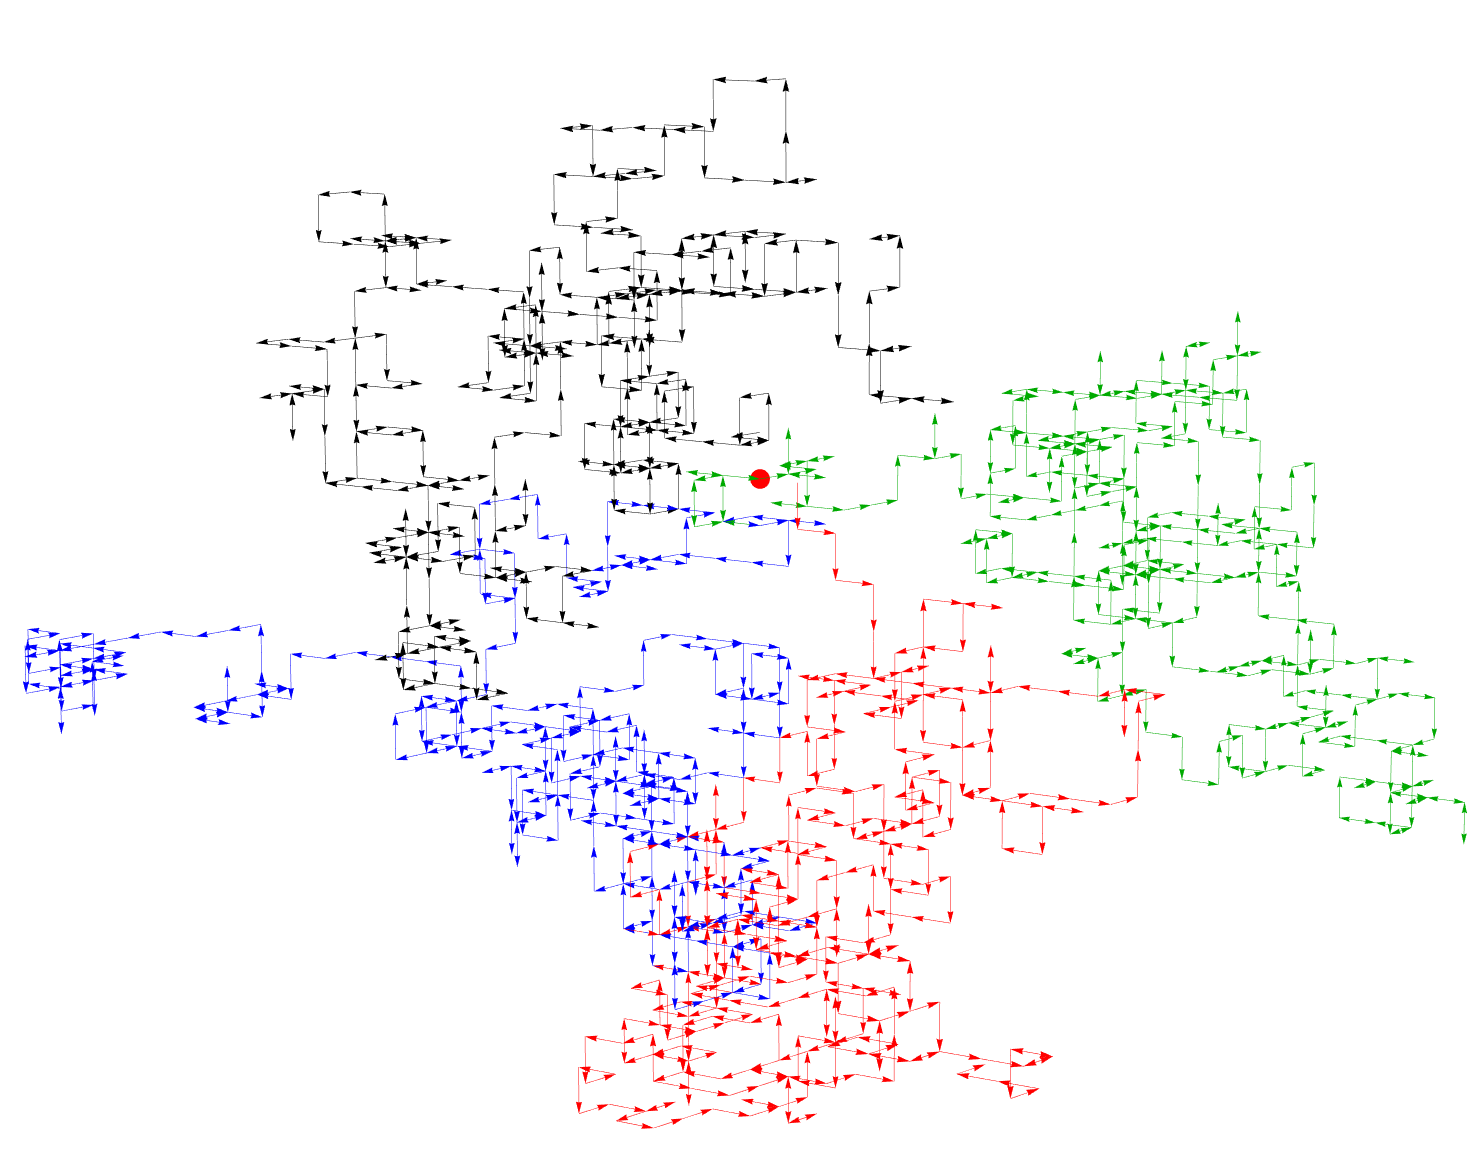
\includegraphics[width=\linewidth]{Figures/quantum-walks/3d-randomwalk.png}
%     \caption{Example of three random walks on $\ZZ^3$.}
% \end{wrapfigure}
% conversionRules = {1 -> {1, 0}, 2 -> {0, 1}, 3 -> {-1, 0}, 
%    4 -> {0, -1}};
% conversionRules3D = {1 -> {1, 0, 0}, 2 -> {0, 1, 0}, 3 -> {0, 0, 1}, 
%    4 -> {0, 0, -1}, 5 -> {0, -1, 0}, 6 -> {-1, 0, 0}};
% makeSteps[num_] := RandomInteger[{1, 4}, num] /. conversionRules;
% makeSteps3D[num_] := RandomInteger[{1, 6}, num] /. conversionRules3D;
% Graphics3D[{
%   {Red, PointSize@0.01, Point@{0, 0, 0}},
%   {Black, Arrowheads@0.005, 
%    Arrow /@ Most@Transpose@{#, RotateLeft@#} &@
%     Accumulate@makeSteps3D@400},
%   {Red, Arrowheads@0.005, 
%    Arrow /@ Most@Transpose@{#, RotateLeft@#} &@
%     Accumulate@makeSteps3D@400},
%   {Blue, Arrowheads@0.005, 
%    Arrow /@ Most@Transpose@{#, RotateLeft@#} &@
%     Accumulate@makeSteps3D@400},
%   {Darker@Green, Arrowheads@0.005, 
%    Arrow /@ Most@Transpose@{#, RotateLeft@#} &@
%     Accumulate@makeSteps3D@400}
%   },
%  (*PlotRange\[Rule]ConstantArray[{-25,25},3],Axes\[Rule]True*)
%  
%  PlotRange -> All, Boxed -> False
%  ]


% \tmpHeading{They are time-homogeneous MCs}
% The fact that the transition probability does not depend neither on the time $t$ nor on the previous history of the walker, but rather it depends exclusively on the current position, is a crucial properties of random walks, that characterises them as \textit{time-homogeneous Markov chains},
% \footnote{A \textit{Markov chain}, or \textit{Markov process}, is a generic type of stochastic process in which the probability of each event only depends on the state of the system at the previous time, rather than on the entire history of the system. Random walks are a notable example of Markov process.}
% which is a more general class of memoryless stochastic processes.

% \tmpHeading{Transition matrix}
% We can collect the set transition probabilities into a matrix $M$. This matrix will then be a \textit{bistochastic matrix}, that is a matrix satisfying $\sum_i M_{ij}=\sum_j M_{ij}=1$. If we collect the set of transition probabilities of going from $i$ to $j$ in the $i$-th column of $M$, we can then write compactly the evolution of a walk in linear algebraic notation as
% \begin{equation}
%     P_{k+1} = M P_k = M^k P_0,
% \end{equation}
% where $P_k$ is the vector of probabilities at the set $k$ ($(P_k)_i$ is the probability of finding the walker at the position $i$ at the $k$-th step).


\tmpHeading{Quantum walks}
\acp{QW} are models of quantum dynamics which share many similarities with classical random walks, and are often understood as their quantum counterparts~\cite{aharonov2000quantum,kempe2003quantum,venegasandraca2012quantum,portugal2013quantum}.
We here discuss exclusively \emph{discrete-time} \acp{QW}~\cite{chandrashekar2008optimizing}, which bear the most direct analogy with classical random walks, and will always refer to these when mentioning ``QWs''.
In its simplest form, a \ac{QW} involves a high-dimensional system, usually referred to as \emph{walker}, endowed with an inner $2$-dimensional degree of freedom, referred to as the \emph{coin}, in analogy with the classical case.
Like classical random walks, QWs are defined on graphs in the general case~\cite{aharonov2000quantum}, but here we only discuss QWs \emph{on a line}. These are QWs in which the walker can only move in one of two directions, say ``left'' and ``right''~\cite{ambainis2001onedimensional}.
A single \textit{step} of such a discrete-time \ac{QW} consists of a unitary evolution applied to the current state of the \ac{QW}. The time is therefore \emph{discrete} in the sense that there is no notion of ``time'' as a continuous parameter. Rather, the state changes by discrete amounts at each step, just as its classical counterpart.

% \tmpHeading{Discrete and continuous QWs}
% A first important distinction is between \textit{discrete} and \textit{continuous} \acp{QW}.
% Discrete-time QWs are systems comprised of a low-dimensional degree of freedom, usually referred to as the \textit{coin}, coupled with a high-dimensional one named the \textit{walker}.
% In this model, the time is discrete in the sense that the state evolves in discrete \textit{jumps}, rather than evolving continuously in time.
% A different model is the so-called \ac{CTQW}. Here, the dynamics is instead governed by a standard Schr\"odinger equation, and the process is therefore defined via some Hamiltonian. In a \ac{CTQW} there is no place for the notion of a \textit{coin} degree of freedom, which makes the structure of these kinds of model rather different, at least on the surface, from their discrete counterparts\highlight{(maybe mention equivalence between discrete and continuous models)}.

\tmpHeading{QWs for quantum algorithms?}
In contrast with the classical case, QWs evolve \textit{coherently}, bringing interference effects into the picture.
% \acp{QW} have proven useful for quantum algorithm developments, and find multiple uses to develop quantum search algorithms~\cite{ambainis2011search,ambainis2008quantum,ambainis2010developments,kempe2003quantum,kendon2006random,santha2008quantum,venegasandraca2012quantum,venegasandraca2008quantum}.
Both discrete- and continuous-time \acp{QW}  have been shown to be universal for quantum computation~\cite{childs2009universal,childs2013universal},
and allow for efficient implementations of quantum search algorithms~\cite{shenvi2003quantum,ambainis2005coins,tulsi2008faster}.
This led to several experimental implementations~\cite{manouchehri2014physical}, including with atomic systems~\cite{cote2006quantum,schwartz2007transport,chandrashekar2008quantum,perets2008realization,weitenberg2011singlespin,giuseppe2013einsteinpodolskyrosen,fukuhara2013microscopic,meinert2014observation,preiss2015strongly}, trapped ions~\cite{karski2009quantum,schmitz2009quantum,zhringer2010realization}, and photonics systems~\cite{peruzzo2010quantum,rohde2011multi,owens2011twophoton,poulios2014quantum,chapman2016experimental,caruso2016fast}.
% \acp{QW} have been successfully implemented~\cite{manouchehri2014physical} in systems as diverse as trapped atoms~\cite{cote2006quantum}, trapped ions~\cite{schmitz2009quantum,zhringer2010realization}, photonics circuits~\cite{perets2008realization,peruzzo2010quantum,broome2010discrete,schreiber2010photons,rohde2011multi,sansoni2012twoparticle,boutari2016large,cardano2015quantum,cardano2016statistical,caruso2016fast}, and optical lattices~\cite{meinert2014observation}.
In particular, photonics platforms include linear optical interferometers~\cite{sansoni2012twoparticle,crespi2013anderson,harris2015bosonic,pitsios2016photonic}, intrinsically stable multi-mode interferometers with polarization optics~\cite{broome2010discrete,kitagawa2012observation,vitelli2013joining}, fibre-loop systems for time-bin encoding~\cite{schreiber2010photons,schreiber2012a,boutari2016large}, and \acp{QW} in the \ac{OAM} space~\cite{cardano2015quantum,cardano2016statistical}.

\tmpHeading{How we use QWs}
\add{QW dynamics can be implemented in a variety of platforms, thanks to the simplicity of the interaction they require~\cite{manouchehri2014physical}.
It is, however, still subject of active research the full extent to which QWs can be leveraged to control the evolution of a quantum state. In particular, in the context of state engineering, it is not known what kind of quantum states can result from a QW. Owing to the relative easiness of realising QW dynamics, such a result would significantly enlarge the class of realisable states across different experimental platforms.
We will address this issue in~\cref{chapter:quantum_walks}, presenting a complete characterisation of the possible outputs of one-dimensional QWs with time-dependent coin operations.
We then proceed to use this result to experimentally engineer target qudits in the orbital angular momentum of single photons~\cref{chapter:experimental_engineering_qudits}, and showcase ML algorithms to analyse them in~\cref{chapter:ML_VVBs}.}
% QWs will be used in~\cref{chapter:quantum_walks,chapter:experimental_engineering_qudits,chapter:ML_VVBs}. We characterise the possible outputs of time-dependent QWs in~\cref{chapter:quantum_walks}, use this result to engineer target qudits in~\cref{chapter:experimental_engineering_qudits}, and showcase ML algorithms to analyse them in~\cref{chapter:ML_VVBs}.

